\documentclass[a4paper,10pt]{report}

\usepackage[utf8]{inputenc}
\usepackage{hyperref}
\usepackage{graphicx}
\usepackage{color}
\usepackage{array}
\usepackage{eurosans}

% Title Page
\title{Bicing}
\author{Tomas Barton and Mauro Donadeo}


\begin{document}
\maketitle

% \begin{abstract}
% \end{abstract}

\chapter{Introduction}
The aim of this project is to provide an program which would help provider of local bicing service\footnote{Bicing Barcelona -- \url{http://www.bicing.com}} with distribution of bikes to a approach to an ideal state when each user of this service would find a bike when is needed. 

\section{About Bicing}
The Bicing project is quite new in Barcelona, but after few months it became very popular. Owner of a special card, which can be purchased for 30 \euro, can rent a bike from a station for free, if he return this bike to some station in half an hour. Otherwise he pays a few cents for each hour until is the bike returned. 

\begin{figure}[ht]
\begin{center}
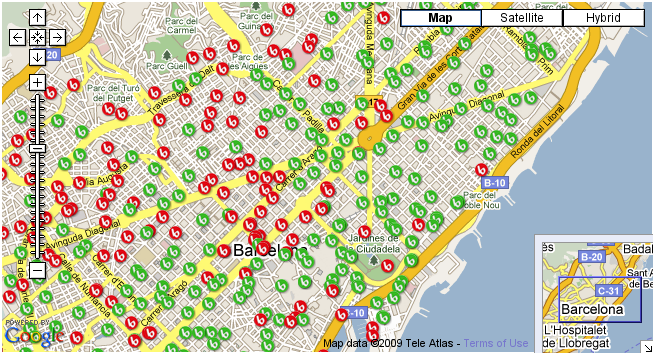
\includegraphics[width=\textwidth]{images/bicing_map.png}
\caption{Map of bicing stations in Barcelona -- red stations are without bikes}
\label{img:bicing_map}
\end{center}
\end{figure}

Nowadays there are more than 400\footnote{418 stations at 12 October 2009} bike stations in Barcelona, the highest concentration of bike stations is of course in centre of city. Usually each station has from 20 up to 30 stands for bikes. In the very center they are placed quite close to each other.



\section{Our task}
With usage of \textbf{\textsl{F}} vans we are supposed to optimize distribution of bikes, so that as many customers as possible will find a disposable bike at time when they need it.

Implementation will be done in Java, we took advantage of AIMA framework, which contains most of algorithm commonly used for local search.

\chapter{Implementation}
\section{State representation} 
Each state must contain information about distribution of bikes over all stations. So that we have to keep:
\begin{itemize}
\item current number of bikes at the station
\item number of bikes that is going to be at station in next hour (moved by users)
\item expected demand for bikes in an hour
\end{itemize}
These information is different for each state, moreover we have other information which we need but it is same for every state:
\begin{itemize}
 \item number of stations
 \item coordinates of stations
\end{itemize}


\section{Operators}


\clearpage
\begin{thebibliography}{9}
\bibitem{fold}{\em Milissa Tarquini:}{\bf Blasting the Myth of the Fold}
		\url{http://www.boxesandarrows.com/view/blasting-the-myth-of} \\
		{This is an electronic document. Date of publication: July 24, 2007. \\
		Date retrieved: January 19, 2009. }


\end{thebibliography}



\end{document}          
